\section{Tervezés és architektúra}

\indent Az alkalmazás fejlesztése során a célkitűzésem az volt, hogy egy jól strukturált, skálázható és hosszú távon is fenntartható rendszert tervezzek, illetve hozzak létre, amely modern fejlesztési elvekre, valamint felhasználói fekületre épül. A rendszer célja, hogy egyszerűsítse a buszjáratok kezelését, a menetrendek nyilvántartását, valamint megkönnyítse a jegyvásárlás és adminisztratív folyamatok végbemenetelét. Ebben a fejezetben bemutatom a rendszer architektúráját, az adatbázis-tervet, az entitások kapcsolatrendszerét, valamint a felhasználói felület tervezése során hozott döntéseket.

\subsection{Rendszerarchitektúra}

\indent Az alkalmazás háromrétegű architektúrát követ, amely a prezentációs, alkalmazáslogikai és adatelérési rétegeket világosan elkülöníti. Ez a struktúra lehetővé teszi a moduláris fejlesztést, a különböző rétegek független tesztelhetőségét, valamint az egyszerű jövőbeli fejlesztésekkel való kibővítést.

\begin{itemize}
    \item \textbf{Prezentációs réteg (View)} – A felhasználói felület ASP.NET MVC technológiával készült, Razor nézetek alkalmazásával. A cél egy átlátható, reszponzív és intuitív felhasználói élmény biztosítása volt. Az oldal struktúrája a Bootstrap keretrendszerre épül, ezzel támogatva a mobileszközökön való megjelenést is.
    
    \item \textbf{Alkalmazáslogikai réteg (Controller + Business Logic)} – Ez a réteg felel az üzleti szabályok érvényesítéséért, az adatok feldolgozásáért és a logikai műveletekért. A kontroller osztályok kommunikálnak az adatelérési réteggel, és ellátják az adatokat a nézetek számára. A rendszer szerepköralapú hitelesítést használ az ASP.NET Identity segítségével.

    \item \textbf{Adatelérési réteg (Data Access Layer)} – Az adatok tárolása SQL Server-ben történik, míg a kommunikáció az Entity Framework Core ORM-en keresztül valósul meg. Ez lehetővé teszi az objektum-orientált adatkezelést, a LINQ-alapú lekérdezéseket és az adatbázis sémájának migrációját.
\end{itemize}

\subsection{Adatbázis-tervezés}

\indent A rendszer adatbázisa relációs sémára épül, amely biztosítja a konzisztens adatkezelést és a gyors lekérdezéseket. A táblák között többféle kapcsolat (egy-a-többhöz, több-a-többhöz) került kialakításra, figyelembe véve a normalizálási szabályokat.
\newpage
\subsubsection{Adatmodell – entitások bemutatása}

Az alábbiakban bemutatom az alkalmazásban használt főbb entitásokat, azok mezőit, adattípusait és a mezők rendeltetését.

\paragraph{Contact}

A \texttt{Contact} entitás a rendszer regisztrált felhasználóit reprezentálja, és az ASP.NET Identity rendszer \texttt{IdentityUser} osztályából származik. Ezáltal örökli annak számos beépített mezőjét és funkcionalitását, mint például a felhasználónév (\texttt{UserName}), e-mail cím (\texttt{Email}), jelszó hash (\texttt{PasswordHash}), valamint a fiók zárolással, biztonsági tokenekkel, e-mail és telefonszám megerősítéssel kapcsolatos mezőket.

\paragraph{Contact}

A rendszer felhasználóit reprezentáló alapvető entitás a \texttt{Contact} osztály, amely az ASP.NET Identity ősosztályára épül, pontosabban az \texttt{IdentityUser} osztályból származik. Ez az öröklődés lehetővé teszi a beépített azonosítási és hitelesítési funkciók használatát, például a felhasználónév, az e-mail cím, a jelszótárolás hash formátumban, valamint a különféle biztonsági funkciók – mint például fiókzárolás, e-mail- és telefonszám-ellenőrzés – elérését.

A projekt specifikus igényeihez igazodva a \texttt{Contact} entitás további mezőkkel került kibővítésre. Minden felhasználó egy egyedi azonosítóval rendelkezik, amely GUID formátumban kerül tárolásra, ez biztosítja az entitás egyértelmű beazonosíthatóságát. A felhasználók teljes neve külön mezőben kap helyet, amely az azonosításon túl a különböző nézetekben és riportokban való megjelenítést is szolgálja. A rendszer az e-mail címet elsődleges kapcsolattartási pontként használja, emellett lehetőség van telefonszám megadására is, amely főként közvetlen kommunikáció esetén hasznos. Az egyes felhasználók szerepköre – legyen az például adminisztrátor, munkatárs vagy ügyfél – szöveges formában kerül rögzítésre, ez határozza meg, hogy milyen jogosultságokkal rendelkeznek a rendszerben. A jelszavak biztonságos tárolását a keretrendszer által biztosított hash-elési mechanizmus kezeli.

A hozzáférések szabályozása szerepkör-alapú logikát követ, így minden felhasználó csak az általa betöltött szerephez tartozó funkciókat érheti el. Bár az ASP.NET Identity rendszer lehetőséget kínál összetettebb jogosultságmodellek kialakítására az \texttt{IdentityRole} és \texttt{UserRole} entitásokon keresztül, a jelen fejlesztés során egy egyszerűsített megoldás került alkalmazásra, amelyben a szerepkörök egyetlen szöveges mezőben kerülnek tárolásra.

A regisztráció, bejelentkezés, jelszómódosítás, illetve a biztonsággal kapcsolatos funkciók – mint például az e-mail visszaigazolás vagy a többszöri sikertelen belépési kísérlet utáni fiókzárolás – mind az ASP.NET Identity keretrendszer alapvető elemeire épülnek. Ezáltal biztosított a felhasználói adatok megbízható kezelése és a rendszerbe való belépések megfelelő védelme.


\paragraph{Bus}

A \texttt{Bus} entitás az egyes autóbuszokat írja le. A \texttt{BusId} (\textit{string}) az egyedi azonosító, míg a \texttt{LicensePlate} mező (\textit{string}) a busz rendszámát tartalmazza. A \texttt{Capacity} mező (\textit{int}) az ülőhelyek számát rögzíti, a \texttt{BusType} mező (\textit{string}) pedig a jármű típusát jelzi, például városi vagy távolsági busz.

\paragraph{Stop}

A \texttt{Stop} entitás egy-egy megállóhelyet reprezentál. Az \texttt{StopId} mező (\textit{string}) az adott megálló egyedi azonosítója. A \texttt{Name} mező (\textit{string}) a megálló nevét, míg a \texttt{Latitude} és \texttt{Longitude} mezők (\textit{double}) a földrajzi koordinátákat – szélességi és hosszúsági adatokat – tárolják.

\paragraph{TransportRoute}

A \texttt{TransportRoute} entitás egy közlekedési útvonalat reprezentál. A TransportRouteId mező (\textit{string}) az útvonal egyedi azonosítója, a \texttt{Name} mező (\textit{string}) pedig az útvonal nevét tartalmazza. A \texttt{StartStopId} és \texttt{EndStopId} mezők (\textit{string}) az induló és végállomások azonosítóit rögzítik.

\paragraph{RouteStop}

A \texttt{RouteStop} entitás egy kapcsolatot képez a megállók és az útvonalak között, ezzel lehetővé téve az egyes útvonalakhoz tartozó megállók sorrendjének meghatározását. Az \texttt{RouteStopId} (\textit{string}) azonosítja az entitást, a \texttt{TransportRouteId} (\textit{string}) a kapcsolódó útvonalra, míg a \texttt{StopId} (\textit{string}) az adott megállóra mutat. Az \texttt{Order} mező (\textit{int}) az adott megálló sorszámát jelzi az útvonalon belül.

\paragraph{Schedule}

A \texttt{Schedule} entitás a menetrendi adatokat tárolja. Az \texttt{ScheduleId} mező (\textit{string}) az egyedi azonosító, a \texttt{TransportRouteId} (\textit{string}) és \texttt{BusId} (\textit{string}) mezők a kapcsolódó útvonalat és autóbuszt azonosítják. A \texttt{DepartureTime} mező (\textit{DateTime}) az indulás pontos időpontját rögzíti.

\paragraph{Ticket}

A \texttt{Ticket} entitás az utasok által megvásárolt jegyeket reprezentálja. A \texttt{TicketId} mező (\textit{string}) az egyedi azonosító, a \texttt{ScheduleId} (\textit{string}) a kapcsolódó menetrendre, a \texttt{PassengerId} (\textit{string}) pedig a jegyet vásárló utasra (Contact) hivatkozik. A \texttt{SeatNumber} mező (\textit{int}) az adott jegyhez tartozó ülőhely számát, míg a \texttt{PurchaseDate} (\textit{DateTime}) a vásárlás időpontját tartalmazza.

\paragraph{AdminMessage}

Az \texttt{AdminMessage} entitás a látogatók vagy felhasználók által küldött üzeneteket tárolja. Az \texttt{AdminMessageId} mező (\textit{string}) az egyedi azonosító, a \texttt{Name} és \texttt{Email} mezők (\textit{string}) az üzenet küldőjének nevét és e-mail címét tartalmazzák. A \texttt{Message} mező (\textit{string}) az üzenet szövegét, a \texttt{SentAt} mező (\textit{DateTime}) pedig annak elküldési időpontját rögzíti.

\paragraph{AdminTask}

Az \texttt{AdminTask} entitás az adminisztrátori feladatokat tárolja. Az \texttt{AdminTaskId} mező (\textit{string}) az egyedi azonosító, a \texttt{Title} és \texttt{Description} mezők (\textit{string}) a feladat nevét és részletes leírását tartalmazzák. A \texttt{CreatedAt} mező (\textit{DateTime}) a létrehozás időpontját, míg az \texttt{AssignedToId} mező (\textit{string}) a felelős adminisztrátorra (Contact) történő hivatkozást tartalmazza.

\paragraph{Attachment}

Az \texttt{Attachment} entitás fájlmellékleteket ír le. Az \texttt{AttachmentId} mező (\textit{string}) egyedi azonosítóként szolgál, a \texttt{FileName} (\textit{string}) a feltöltött fájl nevét, a \texttt{FilePath} (\textit{string}) pedig annak szerveren való elérési útját tartalmazza. A \texttt{UploadedAt} mező (\textit{DateTime}) a feltöltés időpontját, míg az \texttt{UploadedById} mező (\textit{string}) a feltöltést végző felhasználóra (Contact) való hivatkozást jelenti.


\subsubsection{Táblakapcsolatok}

A rendszer relációs adatmodellje több különböző típusú kapcsolatot valósít meg az entitások között, figyelembe véve az alkalmazás logikai működését és az adatintegritás követelményeit. A modellben több egy-a-többhöz (1:N) kapcsolat is megtalálható. Például egy regisztrált felhasználó – akit a \texttt{Contact} entitás reprezentál – több jegyet is birtokolhat, tehát a \texttt{Contact} és a \texttt{Ticket} entitások között 1:N típusú viszony áll fenn. Hasonló reláció létezik a \texttt{Bus} és a \texttt{Schedule} entitások között is, mivel egy adott jármű több menetrend szerint is közlekedhet.

Az útvonalakat alkotó megállók sorrendiségét a \texttt{RouteStop} entitás írja le, amely egy-egy megállót és egy-egy útvonalat köt össze. Ez az entitás két darab N:1 kapcsolatot is tartalmaz: minden \texttt{RouteStop} bejegyzés pontosan egy \texttt{Stop} és egy \texttt{TransportRoute} rekordhoz tartozik. Ezzel a struktúrával biztosítható az útvonalak szakaszainak pontos leképezése és a megállók sorrendjének rögzítése.

A \texttt{Schedule} entitás kettős hivatkozással kapcsolódik a \texttt{Bus} és a \texttt{TransportRoute} entitásokhoz. Minden menetrendi bejegyzéshez pontosan egy busz és egy útvonal tartozik, így ezen kapcsolatok mindegyike egy-egy 1:1 vagy 1:N viszonyt jelent, attól függően, hogy az adott jármű vagy útvonal hány különböző időpontban kerül beütemezésre.

\subsection{Entitások részletes modellezése}

Az alkalmazás modelljei világosan elkülönítik az egyes üzleti szereplőket és folyamatokat, az elvárt funkcionalitásnak megfelelő struktúrában. A \texttt{Ticket} entitás minden egyes példánya konkrét kapcsolatban áll egy felhasználóval (\texttt{Contact}) és egy menetrendi bejegyzéssel (\texttt{Schedule}), valamint egy rendszer által generált ülőhelyszámmal. Ez biztosítja a tranzakciók egyértelmű követhetőségét.

Az útvonalakat részletező \texttt{RouteStop} entitás lehetőséget nyújt a megállók sorrendi rendezésére az adott útvonalon belül, amely különösen hasznos a vizuális megjelenítés vagy térképes lekövetés során. A dokumentumok kezelése céljából létrehozott \texttt{Attachment} entitás lehetőséget ad fájlok feltöltésére és rendszerezésére, például adminisztratív vagy ügyfélszolgálati célból. A \texttt{AdminMessage} és \texttt{AdminTask} entitások a háttérrendszert támogató funkciók megvalósítását szolgálják: előbbi az üzemeltetői kommunikációt, utóbbi a feladatok kijelölését és nyomon követését teszi lehetővé.

\subsection{Adatbázis entitásdiagram}

\begin{figure}[H]
    \centering
    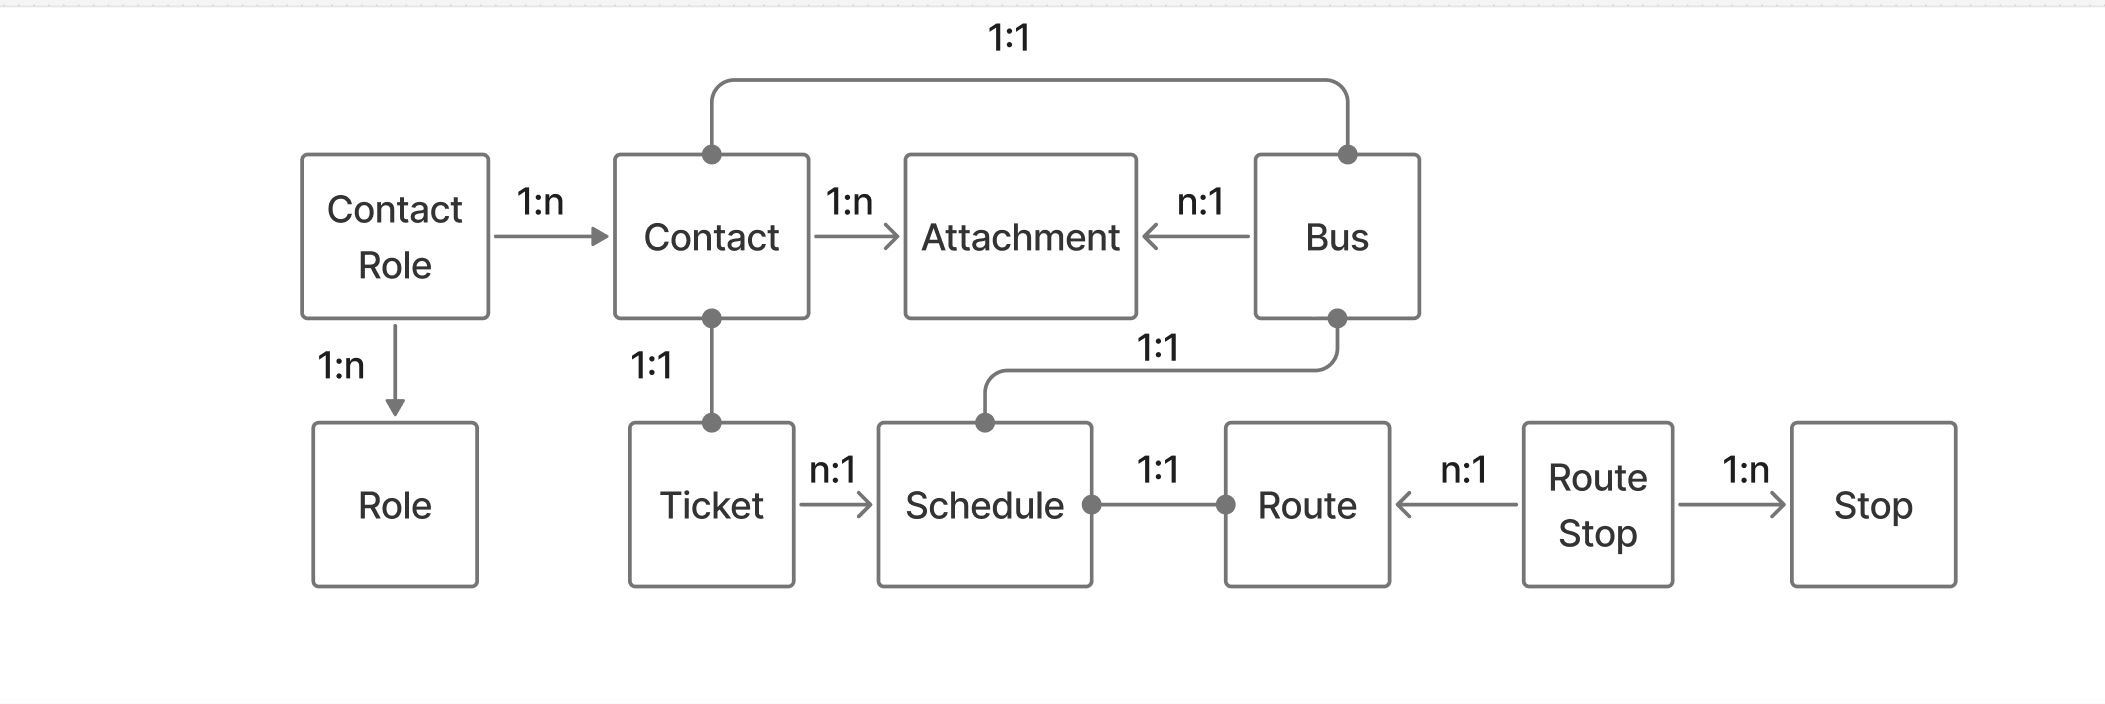
\includegraphics[width=1\textwidth]{Szakdolgozat/Mellekletek/ERdiagram.PNG}
    

    \caption{Az adatbázis entitás-kapcsolat (E-K) diagramja}
    \label{fig:er-diagram}
\end{figure}

A \ref{fig:er-diagram}. ábrán látható az adatbázis logikai struktúrája.


\subsection{Felhasználói felület}

\indent A webalkalmazás felhasználói felületének kialakítása során elsődleges szempont volt az átláthatóság, a reszponzivitás, valamint a felhasználóbarát működés. A rendszer minden látogató számára egységes struktúrát biztosít, azonban a megjelenített tartalom és a hozzáférhető funkciók dinamikusan változnak a bejelentkezési állapot és a felhasználói szerepkör függvényében. A felület úgy került kialakításra, hogy mind a regisztrált utasok, mind az adminisztrátori jogosultsággal rendelkező felhasználók számára a szerepkörükkel releváns tartalom jelenjen meg.

\subsubsection{Főoldal}

\indent A kezdőlap minden látogató számára elérhető, és egy jól strukturált navigációs sávval segíti az alkalmazás fő funkcióinak gyors elérését. A menüsorban az alábbi pontok találhatók meg: \texttt{Stations}, \texttt{Routes}, \texttt{Schedules}, \texttt{MyTickets}, valamint a \texttt{Contact Us}. A jobb felső sarokban megjelenő opciók a látogató aktuális státuszától függenek. Be nem jelentkezett állapotban a \texttt{Login} és \texttt{Register} lehetőségek állnak rendelkezésre, míg bejelentkezett felhasználók esetében a \texttt{Profile} és a \texttt{Logout} gombok válnak láthatóvá. Amennyiben a bejelentkezett felhasználó adminisztrátori jogosultságokkal rendelkezik, egy további \texttt{Adminisztráció} legördülő menü is elérhetővé válik, amely az adminisztrációs funkciókhoz biztosít közvetlen hozzáférést.

\paragraph{Felhasználói nézet (utas szerepkör)}

\indent A rendszer általános felhasználói, azaz az utasok számára kialakított nézet célja, hogy a közlekedési szolgáltatások gyorsan és intuitív módon elérhetők legyenek. A kezdőoldalon keresztül megtekinthetők a vállalat által karbantartott megállók, amelyek földrajzi és logikai elhelyezkedésük alapján rendszerezettek. Az útvonalak menüpont segítségével a felhasználók megismerhetik az elérhető közlekedési útvonalakat, valamint az egyes útvonalakon szereplő megállókat is.

\indent A menetrendek áttekintése szintén kiemelt szerepet kap: az indulási időpontok, a járatokhoz tartozó útvonalak és a járművek együttesen jelennek meg, támogatva a tervezhető és hatékony utazást. A felhasználók számára elérhető a jegyvásárlási lehetőség is, amelyet vizuálisan kiemelt gomb segít megtalálni. A már megvásárolt jegyek a \texttt{MyTickets} szekcióban kerülnek listázásra, ahol a felhasználó saját jegyeit tekintheti át, függetlenül attól, hogy azok aktív vagy már lejárt foglalások. Ezen kívül a \texttt{Contact Us} menüpont egy kapcsolatfelvételi űrlapot biztosít, amelyen keresztül az adminisztráció számára üzenet küldhető, például észrevételek vagy kérdések esetén.

\indent Az egyszerű navigációs élmény részeként a jobb felső sarokban található profilmenü lehetőséget ad a személyes adatok megtekintésére és szerkesztésére. Ezáltal a felhasználók bármikor módosíthatják profiladataikat, illetve kijelentkezhetnek a rendszerből.

\paragraph{Adminisztrátori nézet}

\indent Az adminisztrátorok számára elérhető nézet jelentősen kibővített funkcionalitással rendelkezik. A bejelentkezést követően egy speciális \texttt{Adminisztráció} nevű legördülő menüpont válik aktívvá, amely az alkalmazás háttérrendszeréhez biztosít hozzáférést. Ennek segítségével az adminisztrátorok jogosultak új buszmegállók létrehozására, a meglévő megállók módosítására vagy törlésére. Az útvonalak karbantartása során lehetőség van új útvonalak definiálására, illetve a meglévők struktúrájának frissítésére.

\indent A menetrendek kezelése is része az adminisztrációs felületnek: az indulási időpontokhoz kapcsolódó adatok, valamint a jármű-hozzárendelések módosíthatók. A járműpark menedzselése során az autóbuszok nyilvántartása, adatszerkesztése és bővítése valósítható meg. Az adminisztrátorok hozzáférnek minden felhasználói jegyhez, így átfogó képet kapnak az utazási forgalomról.

\indent A rendszer lehetőséget biztosít a regisztrált felhasználók adatainak kezelésére is, beleértve az egyéni kapcsolattartási információkat és szerepköröket. A \texttt{ToDoList} funkció segítségével az adminisztrátorok belső feladatokat követhetnek nyomon. A beérkező felhasználói üzenetek külön felületen keresztül érhetők el, ahol válaszadásra is van lehetőség.

\indent További fontos adminisztratív funkció a szerepkörök kezelése: az adminisztrátorok új szerepköröket definiálhatnak, illetve módosíthatják a meglévőeket (pl. utas, alkalmazott, adminisztrátor), ezzel szabályozva a hozzáférési jogosultságokat az alkalmazás különböző moduljaihoz.

\indent Míg az utas szerepkörrel rendelkező felhasználók jellemzően csak megtekintési jogosultsággal rendelkeznek, addig az adminisztrátorok számára minden entitáson elérhetővé válik a teljes CRUD-funkcionalitás (Create, Read, Update, Delete). Ez a szerepköralapú jogosultságkezelés biztosítja, hogy a rendszer minden felhasználó számára csak az általa engedélyezett műveletek legyenek elérhetők, miközben a felület egységes marad.
\begin{figure}[H]
    \centering
    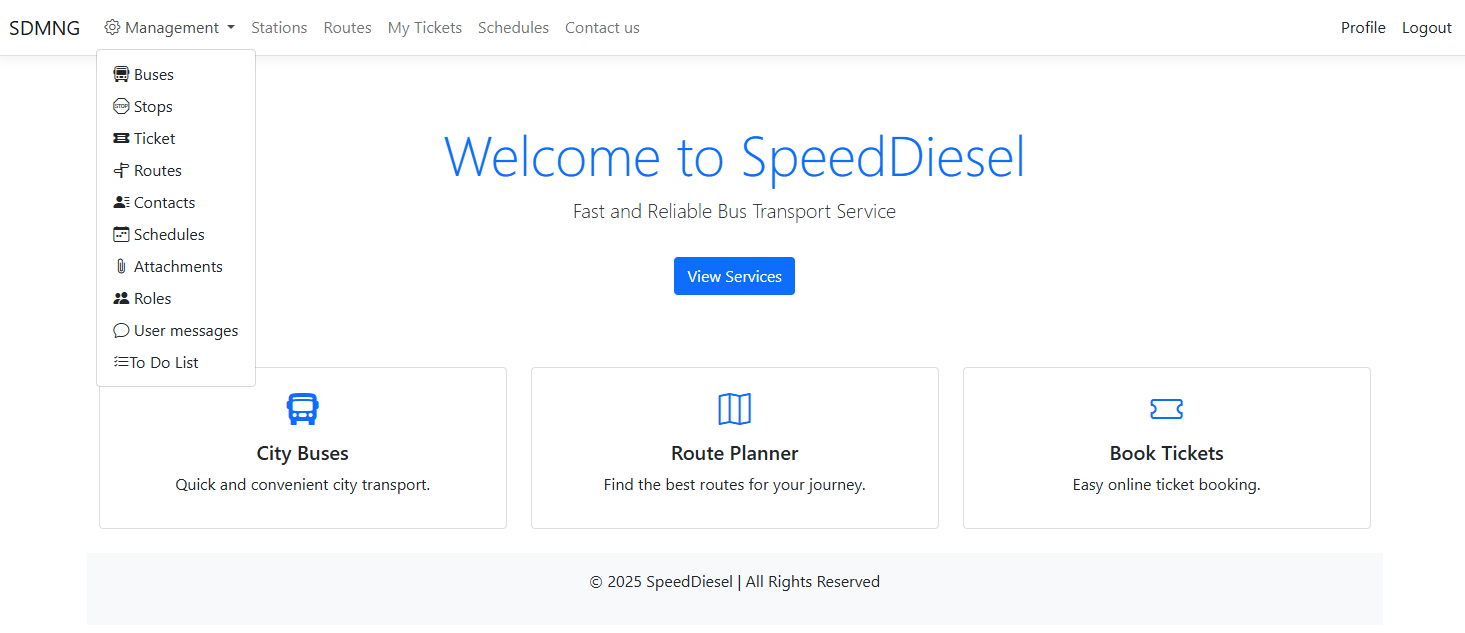
\includegraphics[width=1\textwidth]{Szakdolgozat/Mellekletek/fooldal.PNG}
    \caption{A rendszer főoldala adminisztrátori bejelentkezés után, látható \texttt{Management} menüvel}
    \label{fig:admin-home}
\end{figure}

A \ref{fig:admin-home}. ábra a rendszer főoldalát mutatja be olyan nézetben, amely adminisztrátori jogosultságokkal rendelkező felhasználó számára érhető el. A főmenüsorban jól megfigyelhető a \texttt{Management} lenyíló menüpont, amely kizárólag adminisztrátorok számára jelenik meg. Ezen keresztül elérhetők az adminisztratív funkciók, például megállók, útvonalak, menetrendek és felhasználók kezelése.

\subsubsection{Bejelentkezési oldal (Login)}

A bejelentkezési felületen a felhasználó e-mail címe és jelszava megadásával tud belépni a rendszerbe. Emellett lehetőség van jelszóemlékeztető kérésére is, egy opcionális „Elfelejtett jelszó” linken keresztül. Sikeres bejelentkezést követően a rendszer automatikusan visszairányítja a felhasználót a főoldalra.

\subsubsection{Regisztrációs oldal (Register)}

A regisztrációs oldalon a felhasználó egy egyszerű űrlap kitöltésével hozhat létre új fiókot. Az űrlap a felhasználó nevét, e-mail címét, jelszavát, valamint a szándék megerősítését igényli. A regisztrációt követően a rendszer automatikusan átirányíthatja a bejelentkezési oldalra.

\subsubsection{Stations oldal}

A \texttt{Stations} oldal a rendszer összes regisztrált megállóját listázza. A felhasználói élmény és funkciók a felhasználó szerepkörétől függően változnak, ezért az oldal két különálló nézettel rendelkezik: egy publikus, információs nézettel az utasok számára, valamint egy bővített kezelőfelülettel az adminisztrátorok részére.

\paragraph{Felhasználói nézet (publikus elérés)}

Amennyiben az oldal a főmenüből kerül megnyitásra, a rendszer a látogatók és bejelentkezett utasok számára elérhető változatot jeleníti meg. Ebben a nézetben egy táblázat jelenik meg, amely az összes megállót felsorolja, az alábbi oszlopokkal: \texttt{StopName}, \texttt{Latitude}, \texttt{Longitude}, valamint \texttt{Actions}. Az \texttt{Actions} oszlopban kizárólag egy \texttt{Details} gomb található, amely lehetőséget biztosít az adott megálló részletes adatainak megtekintésére.

A \texttt{Details} gombra kattintva a felhasználó egy különálló nézetre navigál, ahol az adott megálló részletes információi jelennek meg. A felületen szerepel a megálló neve, a földrajzi koordinátái (szélességi és hosszúsági adatok), valamint egy térképes megjelenítés, amely vizuálisan is elhelyezi a megállót a térképen, egy ponttal jelölve annak pontos helyzetét. Ez a nézet teljes mértékben információközlő jellegű, módosítási vagy törlési lehetőséget nem kínál.

\paragraph{Adminisztrátori nézet}

Ha az oldalt az adminisztrációs menüpont \texttt{Stops} almenüjén keresztül nyitjuk meg, a rendszer egy másik nézetet jelenít meg, amely kifejezetten az adminisztrátori szerepkörrel rendelkező felhasználók számára lett kialakítva. Ez a felület nemcsak az adatok megtekintését teszi lehetővé, hanem adminisztratív műveletek végrehajtását is engedélyezi. A táblázatos elrendezés ebben a nézetben megegyezik a publikus nézet szerkezetével — ugyanazok az oszlopok jelennek meg (\texttt{StopName}, \texttt{Latitude}, \texttt{Longitude}, \texttt{Actions}) —, azonban az \texttt{Actions} oszlopban több lehetőség is elérhető. A \texttt{Details} gomb mellett megjelennek a \texttt{Edit} és \texttt{Delete} gombok is, amelyekkel a megálló adatainak szerkesztése, illetve törlése valósítható meg.

Ezen kívül az adminisztrátorok számára elérhető egy \texttt{Create New Stop} gomb is, amely új megállók hozzáadására szolgál. Fontos kiemelni, hogy az adminisztrátorok hozzáférnek a publikus részletező nézethez is, így ők is megtekinthetik ugyanazt az információgazdag, térképes megjelenítést, amely a látogatók és utasok számára is elérhető. Ez lehetővé teszi számukra, hogy a szerkesztési vagy törlési műveletek előtt pontosan ellenőrizzék a megállók földrajzi elhelyezkedését.

Mindkét nézet ugyanazt az adatstruktúrát használja a megállók megjelenítésére, azonban a funkcionális lehetőségek jelentősen eltérnek a felhasználói szerepkörtől függően. A kialakítás célja, hogy egy átlátható, könnyen kezelhető felületet biztosítson mind az információra kíváncsi utasok, mind pedig az adminisztratív műveleteket végző rendszerkezelők számára.

\begin{figure}[H]
    \centering
    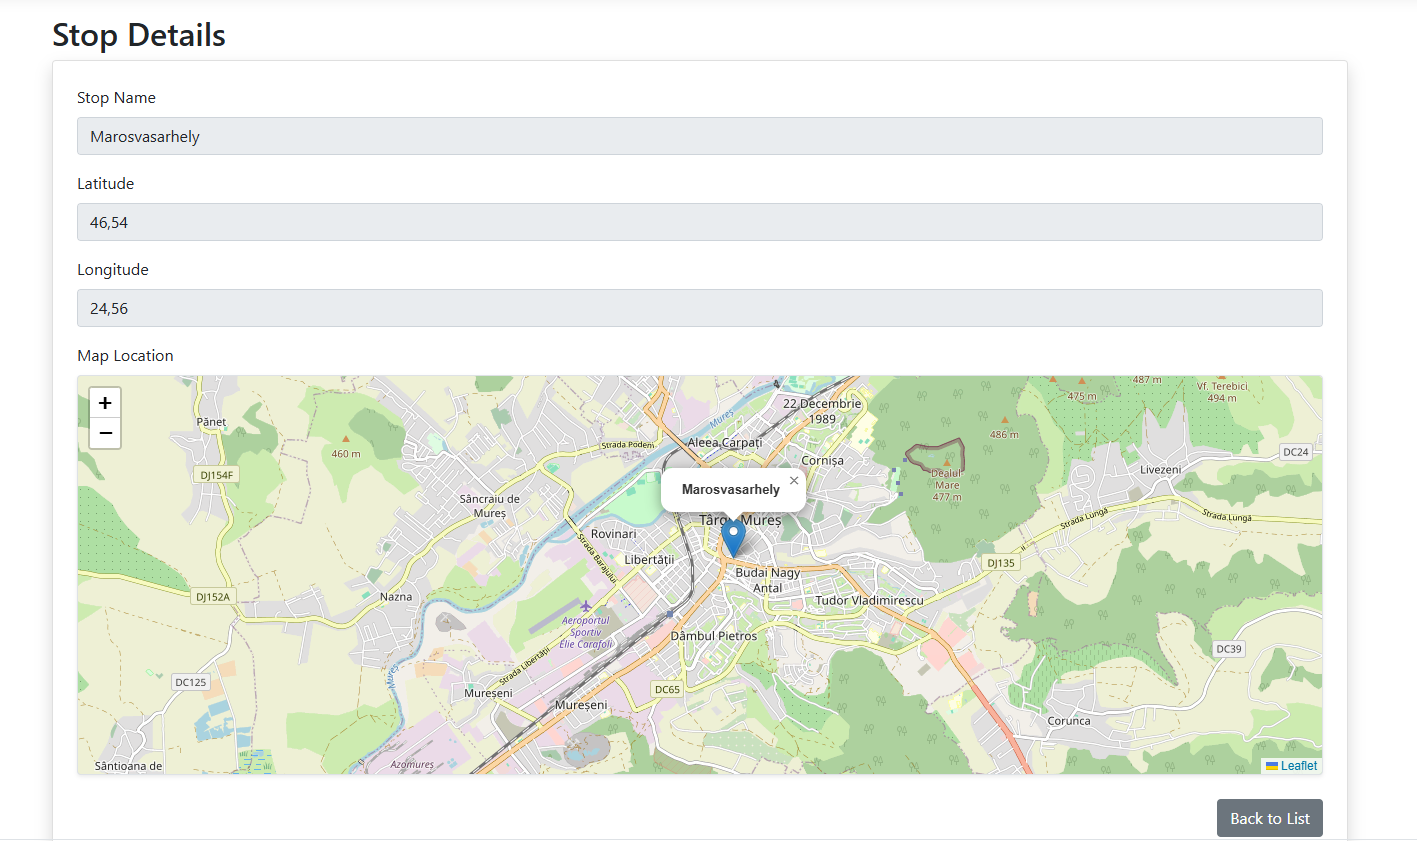
\includegraphics[width=1\textwidth]{Szakdolgozat/Mellekletek/StopDetail.PNG}
    \caption{Megálló részletes adatlapja felhasználói nézetben, térképes megjelenítéssel}
    \label{fig:stop-detail-user}
\end{figure}

A \ref{fig:stop-detail-user}. ábra egy megálló részletes adatlapját szemlélteti olyan formában, ahogyan azt egy általános felhasználó látja, aki a főmenüből navigált erre az oldalra.

Fontos megjegyezni, hogy adminisztrátori jogosultság esetén az ugyanilyen részletes nézet tartalmilag hasonló, azonban a térképes megjelenítés hiányzik belőle. Mivel az adminisztrátorok a megállók kezelését más, célzott nézetekből végzik (pl. a kezelőfelület táblázatos listájából kiindulva), a részletes oldal csupán kiegészítő információként szolgál számukra.


\subsubsection{Routes oldal}

A \texttt{Routes} oldalon a rendszer az adatbázisban szereplő összes elérhető útvonalat listázza. Ennek a felhasználói felület azért szükséges, hogy a látogatók és regisztrált utasok könnyen áttekintést kapjanak az egyes útvonalakról, míg az adminisztrátorok számára részletes kezelési lehetőségeket is biztosít.

\paragraph{Felhasználói nézet (publikus elérés)}

Amennyiben az oldalt a főmenüből érjük el, a rendszer a látogatók és bejelentkezett utasok számára elérhető nézetet jeleníti meg. A megjelenő táblázat az alábbi oszlopokat tartalmazza: \texttt{Name} (az útvonal megnevezése), \texttt{Stops} (egész számként jelölve, hogy hány megállót tartalmaz az adott útvonal), valamint az \texttt{Actions} oszlop, amely egyetlen \texttt{Details} gombot tartalmaz. A felhasználók ezen keresztül tekinthetik meg az adott útvonal részletes információit.

A \texttt{Details} gombra kattintva a felhasználó egy részletes nézethez jut, amely az adott útvonalra vonatkozó információkat jeleníti meg. Az oldal felső részén látható az útvonal neve, alatta pedig egy térkép, amely vizuálisan ábrázolja a megállókat összekötő vonal mentén az útvonalat. A térképet követően egy táblázat jelenik meg, amely sorolja a megállók sorrendjét (\texttt{Index}), nevét, földrajzi szélességi és hosszúsági koordinátáit. Ez a felület kizárólag az információk megtekintésére szolgál, szerkesztési vagy módosítási lehetőséget nem kínál.

\paragraph{Adminisztrátori nézet}

Amennyiben az oldalt az \texttt{Adminisztráció} menüpont \texttt{Routes} opcióján keresztül nyitjuk meg, a rendszer egy adminisztrátori funkciókkal bővített nézetet tölt be. A megjelenő táblázat szerkezete megegyezik a publikus változattal (\texttt{Name}, \texttt{Stops}, \texttt{Actions}), azonban az \texttt{Actions} oszlopban nemcsak a \texttt{Details}, hanem az \texttt{Edit} és \texttt{Delete} gombok is elérhetők, lehetővé téve az útvonalak módosítását vagy törlését. A táblázat felett egy \texttt{Create New Route} gomb is található, amely új útvonalak létrehozására szolgál.

Az adminisztrátor által megnyitott részletes nézet az útvonalhoz rendelt megállókat egy belső táblázatban sorolja fel. Itt az egyes sorok a megállók sorrendi sorszámát, nevét, valamint földrajzi koordinátáit tartalmazzák. A táblázat ezen felül egy \texttt{Actions} oszlopot is tartalmaz, ahol minden megálló mellett elérhető egy \texttt{Delete} gomb. Ennek segítségével az adott megálló eltávolítható az útvonalból, anélkül hogy maga a megálló törlődne az adatbázisból. A táblázat alatt egy lenyíló mező és egy \texttt{Add Stop to Route} gomb található, amelyek új megálló hozzárendelését teszik lehetővé az adott útvonalhoz.

\begin{figure}[H]
    \centering
    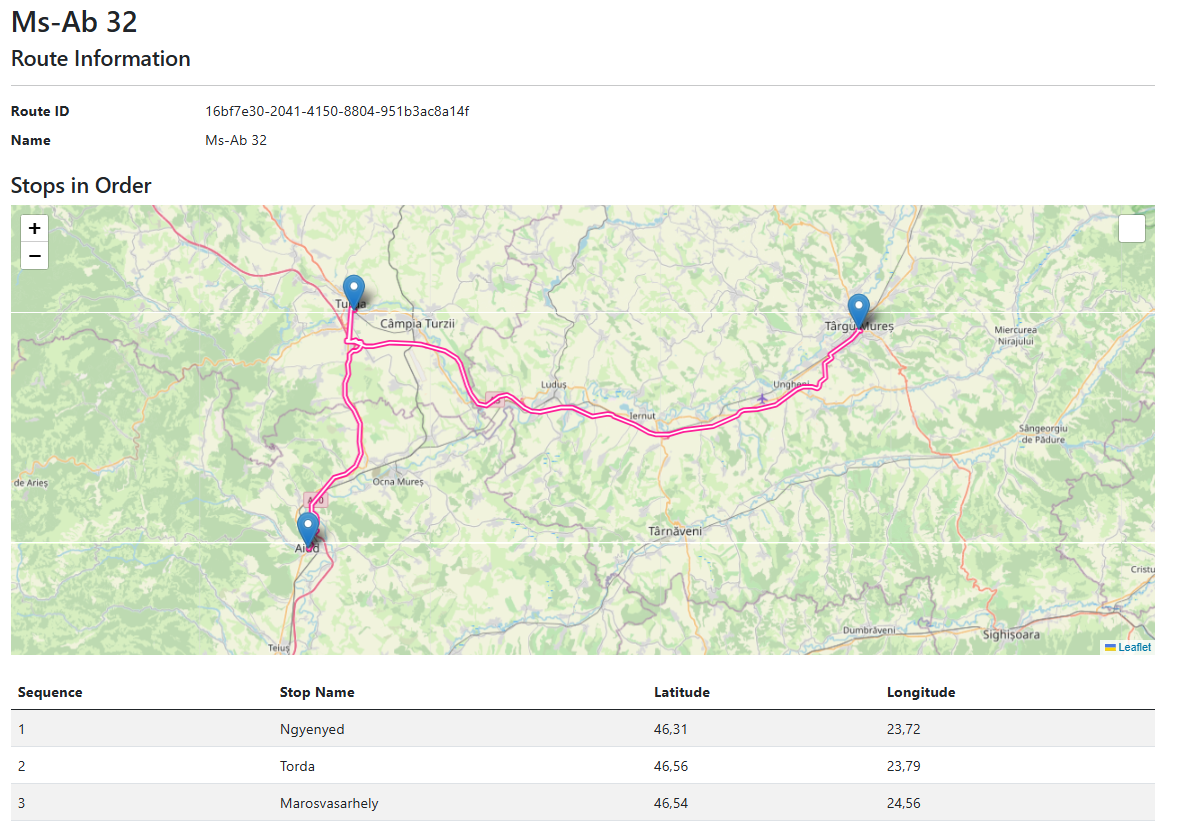
\includegraphics[width=1\textwidth]{Szakdolgozat/Mellekletek/RoutesDetail.PNG}
    \caption{Útvonal részletes adatlapja felhasználói nézetben, térképes megjelenítéssel}
    \label{fig:route-detail-user}
\end{figure}

A \ref{fig:route-detail-user}. ábra egy útvonal részletes adatlapját mutatja be, ahogyan azt egy bejelentkezett felhasználó látja, aki a főmenüből navigált az adott útvonal információihoz. Az adott példában a Nagyenyed–Torda–Marosvásárhely útvonal vizualizációja figyelhető meg.


\subsubsection{Schedules oldal}

A \texttt{Schedules} oldalon a felhasználók a menetrendeket böngészhetik, amelyeket dátum, időpont, útvonal és a közlekedő busz szerint csoportosít a rendszer. Amennyiben az adott járaton van szabad ülőhely, lehetőség van jegyvásárlásra is. Az adminisztrátorok teljes körű menetrendkezelést végezhetnek: új menetrendeket adhatnak hozzá, szerkeszthetik vagy törölhetik a meglévőket, valamint hozzárendelhetik a kiválasztott útvonalakat és autóbuszokat.

\subsubsection{MyTicket oldal}

A \texttt{MyTicket} oldal célja a rendszerben rögzített jegyvásárlások megjelenítése és áttekintése. Az oldal két különböző nézetet biztosít a felhasználói szerepkör függvényében: egyet az általános felhasználók (utasok), egy másikat pedig az adminisztrátorok számára. 

\paragraph{Felhasználói nézet (utasok részére)}

Amennyiben egy bejelentkezett felhasználó navigál a \texttt{MyTicket} oldalra, a rendszer kizárólag az adott személyhez tartozó jegyeket jeleníti meg. A felületen egy táblázat látható, amely a következő oszlopokat tartalmazza: \texttt{TicketId}, \texttt{PurchaseDate}, \texttt{SeatNumber}, \texttt{User} (automatikusan az aktuális felhasználó), \texttt{Schedule}, valamint az \texttt{Actions} oszlop. Az \texttt{Actions} oszlopban egyetlen műveletgomb kap helyet: a \texttt{Details}, amely az adott jegy részletes adatlapjára irányít.

A \texttt{Details} nézetben a felhasználó bővebb információkat kap a jegyhez tartozó menetrendről, beleértve az indulási és érkezési állomásokat, a járat buszának rendszámát, illetve megjelenik egy interaktív térkép is, amely az utazás útvonalát vizuálisan ábrázolja. Ez az ábra segíti az utasokat az útvonal pontos áttekintésében, és kiegészíti az egyéb szöveges információkat.

\paragraph{Adminisztrátori nézet}

Az adminisztrátorok számára a \texttt{Tickets} oldal a \texttt{Management} menüponton keresztül érhető el, ahol az összes, a rendszerben rögzített jegy megjelenik, függetlenül attól, hogy mely felhasználó vásárolta meg őket. Az itt található táblázat szerkezete megegyezik a felhasználói nézettel, azzal a különbséggel, hogy a \texttt{User} oszlopban minden jegyhez tartozó felhasználó kiléte is feltüntetésre kerül. Ez lehetővé teszi az adminisztrátorok számára a jegyek teljes körű nyomon követését és kezelését.

A táblázat \texttt{Actions} oszlopában három funkciógomb található: \texttt{Details}, \texttt{Edit} és \texttt{Delete}. A \texttt{Details} gombbal megnyitható a jegy részletes adatlapja, ahol bővebb információk jelennek meg az adott utazásról, míg az \texttt{Edit} és \texttt{Delete} gombokkal az adminisztrátor módosíthatja vagy törölheti az adott jegyet. Ezzel biztosított a teljes adminisztratív kontroll az összes jegy felett.

Az admin nézet részletes felülete struktúrájában hasonló a felhasználói nézethez, azonban itt nem szerepel a térképes útvonalmegjelenítés. A hangsúly inkább az adatok rendszerezett és pontos bemutatásán van: ide tartoznak az indulási és érkezési megállók, a menetrend adatai, a járat azonosítója és a kapcsolódó felhasználói információk.

Ez az oldal különösen informatív és részletes, összevetve más, jelenleg használatban lévő közlekedési rendszerekkel. Míg sok hasonló alkalmazásban a jegykezelés csupán alapinformációkra szorítkozik, itt az adminisztrátorok számára biztosított minden szükséges funkció a hatékony kezeléshez és ellenőrzéshez.



\subsubsection{Contact Us oldal}

A \texttt{Contact Us} oldal elsődleges célja, hogy lehetőséget biztosítson a látogatók számára az adminisztrátorral való közvetlen kapcsolatfelvételre. Ez az oldal nyilvánosan elérhető, így használatához nincs szükség bejelentkezésre, ami különösen fontos szempont volt a tervezés során. A kapcsolatfelvételi felület egy egyszerűen kezelhető űrlapot tartalmaz, amely négy mezőből áll: a feladó neve (\texttt{Name}), e-mail címe (\texttt{Email}), az üzenet tárgya (\texttt{Subject}) és maga az üzenet tartalma (\texttt{Message}).

A felhasználó az űrlap kitöltését követően a \texttt{Send} gomb segítségével tudja elküldeni az üzenetet. A rendszer a beküldött adatokat automatikusan elmenti az adatbázis megfelelő táblájába, így az adminisztrátorok később visszakereshetik azokat. Emellett a rendszer e-mail értesítést is küld az adminisztrátori címre, amely tartalmazza a megadott adatokat, lehetővé téve a gyors reagálást.

Fontos megjegyezni, hogy ez az oldal kizárólag a felhasználói felületen érhető el, és nem része az admin menüpontoknak. Az alkalmazás ezzel a funkcióval lehetőséget biztosít arra, hogy a látogatók közvetlenül visszajelzést küldjenek, kérdéseket tegyenek fel vagy hibát jelentsenek, így támogatva a folyamatos fejlesztést és felhasználói elégedettséget.

\subsubsection{Adminisztrációs oldalak}

A rendszer adminisztrátori jogosultságokkal rendelkező felhasználói számára külön menüpontok érhetők el a felhasználói felület felső navigációs sávjában található \texttt{Management} legördülő menüben. Ezek a funkciók kizárólag az adminisztrátorok számára hozzáférhetők, céljuk a rendszer különböző erőforrásainak és entitásainak karbantartása és felügyelete.

A menüpontok közül a \texttt{Contacts} oldal tartalmazza a rendszerbe regisztrált összes felhasználót – ideértve az adminisztrátorokat, munkatársakat és általános felhasználókat egyaránt. Az oldal megnyitásakor egy táblázatos nézet fogadja a felhasználót, amely a következő adatmezőket jeleníti meg: \texttt{FullName}, \texttt{Email}, \texttt{Street}, \texttt{Zipcode}, \texttt{Active}, \texttt{Bus}, valamint az \texttt{Actions} oszlop. Az \texttt{Actions} oszlopban három gomb kapott helyet, amelyek lehetővé teszik a kiválasztott felhasználó adatainak részletes megtekintését, szerkesztését vagy törlését (\texttt{Detail}, \texttt{Edit}, \texttt{Delete}). A táblázat alatt egy külön gomb is található, amely új felhasználó manuális hozzáadását teszi lehetővé, ezáltal bővítve az adminisztrátor lehetőségeit a rendszer kézi karbantartása során.

A három elérhető műveleti gomb mindegyike hasonló szerkezetű oldalra navigál, azonban az adott funkciónak megfelelően eltérő célokat szolgál. A részletes megtekintés során az adminisztrátor az adott felhasználó összes adatát áttekintheti egy jól strukturált nézetben, míg a szerkesztés során ezen adatok módosítására is lehetőség nyílik. A törlés funkció egy deaktivációs müvelet legyen, ne töröljünk felhasználókat, csak ideiglenesen legyenek inaktívak.

Minden nézet tartalmazza azokat az információkat, amelyek az adminisztrációs táblázatban is szerepelnek (név, e-mail, cím stb.), azonban ezeken túl két további mező is megjelenik: a felhasználóhoz rendelt szerepkör (\texttt{Role}), valamint az adott felhasználóhoz társított autóbusz megléte vagy hiánya. Ez utóbbi információ különösen fontos a buszvezetői szerepköröknél, mivel ezek a jogosultságok gyakran kapcsolódnak konkrét járművekhez. Az adminisztrátor így átfogó képet kap a felhasználók státuszáról, jogosultságairól és az esetleges operatív hozzárendelésekről is.

A szerkesztési nézet (\texttt{Edit}) további fontos funkcióval is bővül. Ebben a nézetben ugyanis lehetőség nyílik a kiválasztott felhasználó szerepkörének módosítására egy legördülő menü segítségével. Ezáltal az admin dönthet arról, hogy az adott felhasználó egyszerű felhasználó, adminisztrátor vagy más speciális szerepkört töltsön be a rendszerben. Hasonlóképpen, a rendszer lehetőséget biztosít arra is, hogy az admin egy konkrét autóbuszt rendeljen hozzá a kiválasztott felhasználóhoz, amennyiben az adott szerepkör ezt megengedi. Mindkét funkció csak az admin jogosultsággal rendelkező személyek számára érhető el, az általános felhasználók nem tudják ezeket az attribútumokat módosítani, ezáltal garantálva a rendszer adatainak integritását és a jogosultságkezelés biztonságát.

A \texttt{Buses} oldal az adminisztrátorok számára elérhető felület, amely lehetővé teszi a rendszerben nyilvántartott autóbuszok kezelését. Az oldalra lépve egy áttekinthető táblázat fogadja a felhasználót, amely az egyes járművek legfontosabb adatait sorolja fel: \texttt{BusNumber} (rendszám), \texttt{Capacity} (férőhelyek száma), \texttt{BusType} (járműtípus), \texttt{ImageUrl} (a járműhöz tartozó kép elérési útvonala), valamint az \texttt{Actions} oszlop, ahol a megszokott \texttt{Detail}, \texttt{Edit} és \texttt{Delete} gombok segítségével hajthatók végre a különféle műveletek. Ezek az akciók minden esetben a megfelelő, funkcionálisan elkülönített nézetekre vezetnek, ahol a járműadatok megtekintése, módosítása vagy törlése történik.

A táblázat alján elhelyezett gomb egy új autóbusz hozzáadására szolgál, és a \texttt{Create Bus} oldalra navigál, ahol a felhasználónak lehetősége van megadni az új jármű alapadatait: \texttt{BusNumber}, \texttt{Capacity}, valamint a \texttt{BusType}. Ezen kívül egy speciális kiválasztó mező is elérhető, amelynek segítségével hozzárendelhető egy sofőr az adott buszhoz – ez azonban kizárólag admin jogosultság esetén látható és használható. A kiválasztás csak a rendszerben szereplő, megfelelő szerepkörrel rendelkező felhasználók közül történhet.

Az egyes autóbuszokra kattintva elérhető \texttt{Detail} nézet szintén az említett adatokat jeleníti meg, kiegészítve az adott járműhöz rendelt sofőr nevével is. Ez a megjelenítés nemcsak az adminisztratív nyilvántartást könnyíti meg, hanem átláthatóvá teszi a felelősségi viszonyokat is, amely különösen hasznos lehet nagyobb flotta kezelésekor. Ezen kívül a részletes oldalon található egy \texttt{Add Attachment} gomb is, amely egy külön felületre irányít, ahol az adminisztrátor fájlokat – például műszaki dokumentációt vagy engedélyeket – csatolhat a járműhöz egy kiválasztómező segítségével. Ez a kiegészítő funkció lehetővé teszi a dokumentumkezelés központosítását és rendszerezését a járművekhez kapcsolódóan.

Az \texttt{Attachments} oldal az adminisztrátorok számára biztosít hozzáférést a rendszerben tárolt valamennyi melléklethez. Az oldalon egy áttekintő táblázat található, amelyben minden fájlhoz kapcsolódó alapinformáció megjelenik. A felsorolt adatok a következők: \texttt{FileName} (a fájl neve), \texttt{FileType} (típusa), \texttt{UploadDate} (feltöltés dátuma), \texttt{ExpirationDate} (lejárati dátuma), \texttt{FullName} (a melléklethez kapcsolt felhasználó neve), valamint \texttt{BusNumber} (az érintett jármű rendszáma). A \texttt{UploadDate} mindig a tényleges feltöltési időpontot mutatja, míg az \texttt{ExpirationDate} automatikusan egy évvel későbbre kerül beállításra.

A rendszer biztosítja, hogy minden melléklet vagy egy felhasználóhoz (\texttt{Contact}), vagy egy autóbuszhoz (\texttt{Bus}) legyen hozzárendelve – egyszerre azonban csak az egyikhez. Abban az esetben, ha az egyik kapcsolat nem kerül megadásra, az adott mező \texttt{NA} (Not Assigned) értéket kap a táblázatban, ezzel jelezve a hiányzó kapcsolatot.

A táblázat utolsó oszlopában találhatóak az adminisztrációs műveleteket biztosító gombok, nevezetesen a \texttt{Detail}, \texttt{Edit} és \texttt{Delete} opciók, amelyek lehetőséget nyújtanak az adott melléklet adatainak megtekintésére, módosítására vagy törlésére. Ezek a funkciók az admin felhasználók részére elérhetőek, és minden esetben biztosítják a csatolmányok pontos nyilvántartását.

Új melléklet hozzáadására ezen az oldalon nincs lehetőség, mivel a feltöltési művelet kizárólag az érintett felhasználó vagy autóbusz részletes adatlapjáról indítható. Az ott elhelyezett \texttt{Add Attachment} gomb segítségével lehet kiválasztani és csatolni a kívánt dokumentumot, amely ezáltal automatikusan a megfelelő entitáshoz kerül kapcsolásra. Ez a struktúra lehetővé teszi az adatok pontos szervezését és visszakereshetőségét, miközben kizárólag az adminisztrátorok számára biztosítja a hozzáférést és módosítási jogosultságot.

Az \texttt{User Messages} oldal az adminisztrátorok számára készült, és a felhasználóktól érkező kapcsolatfelvételi üzenetek kezelésére szolgál. Ez az oldal a \texttt{Management} menüpont alól érhető el, és tartalmazza az összes olyan bejegyzést, amely a \texttt{Contact Us} űrlap kitöltésével került rögzítésre a rendszerben. A megjelenített táblázat minden üzenetet listáz, függetlenül attól, hogy azokat már megtekintették-e vagy sem.

A táblázat oszlopai a következő információkat jelenítik meg: \texttt{UserName} (a feladó neve), \texttt{UserEmail} (az e-mail címe), \texttt{Subject} (az üzenet tárgya), \texttt{SentAt} (küldés időpontja), valamint az \texttt{IsRead} mező, amely azt jelzi, hogy az adott üzenetet az admin már megnyitotta-e. A rendszer automatikusan nyomon követi az üzenetek megtekintését: amint az adminisztrátor rákattint a \texttt{Detail} gombra és megnyitja az adott bejegyzést, az \texttt{IsRead} értéke automatikusan \texttt{true}-ra változik, így a későbbiekben is egyértelműen nyomon követhető, mely üzenetek lettek már feldolgozva.

Az \texttt{Actions} oszlop egyetlen gombot tartalmaz, amely a részletek megtekintésére szolgál. A megnyitott nézetben az admin elolvashatja a felhasználó által küldött teljes üzenetet. A rendszer nem biztosít lehetőséget ezen üzenetek szerkesztésére vagy törlésére, hiszen ezek kizárólag tájékoztatási célból kerülnek be az adatbázisba.

Fontos kiemelni, hogy ezen az oldalon nem áll rendelkezésre új üzenet manuális hozzáadására szolgáló funkció, mivel az összes bejegyzés kizárólag a felhasználói űrlap kitöltésével jöhet létre. Az oldal célja a felhasználói visszajelzések átlátható, hatékony kezelése és archiválása az adminisztráció számára.

A \texttt{ToDoList} menüpont az adminisztrátorok számára elérhető, és a rendszerben végzendő feladatok kezelését teszi lehetővé. Ez az oldal interaktívabb megközelítést alkalmaz, mint a többi adminisztrációs felület, mivel nem csupán adatokat jelenít meg, hanem lehetőséget biztosít az egyéni feladatok nyomon követésére és kezelésére is.

Az oldal betöltésekor egy áttekinthető táblázat jelenik meg, amely minden korábban létrehozott feladatot tartalmaz. A táblázat három fő oszlopból áll: \texttt{Title} (a feladat címe), \texttt{Due} (a határidő), valamint az \texttt{Actions} oszlop, amely két műveleti gombot tartalmaz. Ezek közül a \texttt{Detail} gomb a feladat részleteit jeleníti meg, míg az \texttt{Edit} gomb közvetlenül a szerkesztőfelületre navigál.

A részletes nézet szintén tartalmaz egy \texttt{Szerkesztés} gombot, amely ugyanarra az \texttt{Edit} oldalra visz tovább. Mind a részletes nézetben, mind pedig a szerkesztőfelületen a feladat alábbi mezői jelennek meg: a cím, a határidő és egy jelölőnégyzet, amellyel a feladat státusza állítható be – ez azt mutatja, hogy a feladat elvégzése megtörtént-e. Ennek a mezőnek a bejelölésével a feladat „készre jelenthető”.

A feladatok vizuálisan is jól elkülöníthetők az állapotuk alapján: a már teljesített feladatokat a rendszer zöld háttérrel jeleníti meg, míg a még el nem végzetteket fehéren emeli ki. Ez a színkódolás segíti az adminokat abban, hogy gyorsan átlássák az aktuális teendőket, és azonnal be tudják azonosítani a sürgős feladatokat.


\begin{figure}[H]
\centering
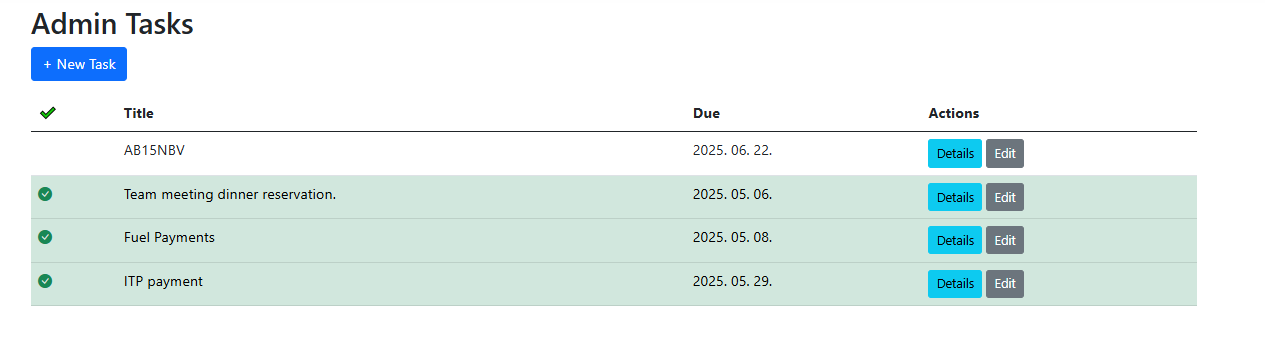
\includegraphics[width=1\textwidth]{Szakdolgozat/Mellekletek/admintasks.PNG}
\caption{Adminisztrátori feladatok listája látható }
\label{fig:todo-admintask}
\end{figure}

A \ref{fig:todo-admintask}. ábra az adminisztrátorok számára elérhető \texttt{ToDoList} oldal listanézetét szemlélteti, ahol az aktuális feladatok áttekinthető formában jelennek meg.